% ============================================================
%  CONCEPTION ET MISE EN ŒUVRE — realisation.tex
% ============================================================
\section{Conception et mise en œuvre}
\label{sec:realisation}

Après avoir établi le référentiel fonctionnel dans la
section~\ref{sec:specification}, cette section décrit la conception logicielle et
son implémentation. Elle explique comment les choix architecturaux répondent aux
exigences du projet et comment le code a été structuré pour garantir
l'extensibilité et la maintenabilité. Les composantes du système sont examinées
successivement~: l'architecture modulaire globale, la hiérarchie des classes de
données, l'interface Homme-Machine et les traitements algorithmiques au cœur du
moteur de simulation.

% ------------------------------------------------------------
\subsection{Architecture globale du logiciel}
\label{subsec:archi_globale}

L'application est organisée en quatre modules distincts selon une architecture
modulaire à responsabilités séparées. La figure~\ref{fig:architecture} représente
cette décomposition ainsi que les dépendances entre modules.

\begin{figure}[htbp]
  \centering
  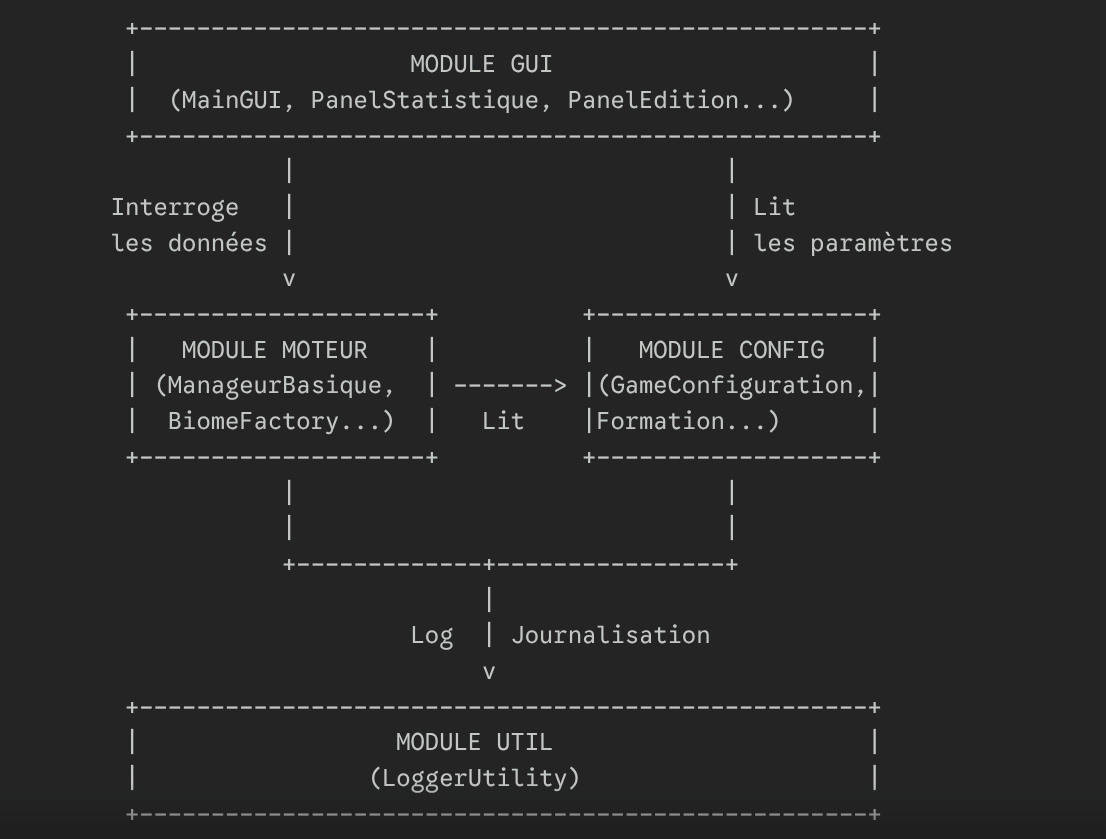
\includegraphics[width=0.85\textwidth]{images/architecture.png}
  \caption{Architecture modulaire de l'application Environnement}
  \label{fig:architecture}
\end{figure}
\needspace{5\baselineskip}
Les quatre modules identifiés dans la figure~\ref{fig:architecture} sont les
suivants.

\begin{itemize}
  \item \textbf{Module \texttt{moteur}}~: constitue le cœur de la simulation. Il
    contient la logique métier~: gestion de la carte, des biomes, des événements
    et des règles de transformation. Ce module est indépendant de l'interface
    graphique et peut fonctionner sans interaction utilisateur.
  \item \textbf{Module \texttt{gui}}~: gère l'interface utilisateur. Il contient
    les classes d'affichage (\texttt{MainGUI}, \texttt{MainDisplayer},
    \texttt{PanelStatistique}, \texttt{PanelTemps}, \texttt{PanelEdition},
    \texttt{TutorielPanel}) et la classe de rendu (\texttt{StrategiePeinture}).
    Ce module dépend du module \texttt{moteur} pour récupérer les données à
    afficher.
  \item \textbf{Module \texttt{config}}~: centralise tous les paramètres~:
    caractéristiques initiales des biomes, effets des événements, seuils de
    transformation et probabilités de génération.
  \item \textbf{Module \texttt{util}}~: regroupe les utilitaires transversaux,
    dont le système de journalisation (\texttt{LoggerUtility}) et la configuration
    Log4j. Il est utilisé par tous les autres modules.
\end{itemize}

Cette séparation en modules garantit que toute modification d'un module n'impacte
  pas les autres, à condition de respecter les interfaces publiques définies. Elle
  facilite également les tests unitaires de chaque composant de manière isolée.

  \paragraph{Positionnement MVC.}
  L'architecture du projet s'articule autour du modèle MVC (Modèle-Vue-Contrôleur).
  Le Modèle (M) correspond au module \texttt{moteur}, qui contient les classes
  \texttt{ManageurBasique}, \texttt{Carte}, \texttt{Biome} et \texttt{Evenement}.
  La Vue (V) est assurée par le module \texttt{gui} via les classes
  \texttt{MainGUI} et \texttt{StrategiePeinture} qui gèrent le rendu graphique.
  Les Contrôleurs (C) sont les Listeners des boutons Swing, qui font le lien entre
  les interactions utilisateur et le moteur de simulation.

% ------------------------------------------------------------
\needspace{15\baselineskip}
\subsection{Classes de données}
\label{subsec:classes_donnees}

Cette sous-section décrit la conception des classes représentant les entités
fondamentales de l'écosystème~: biomes, événements et carte. Elle présente
également les propriétés initiales des biomes, qui constituent un paramètre
central du comportement de la simulation.

\paragraph{Hiérarchie des biomes.}
La classe abstraite \texttt{Biome} constitue la racine de la hiérarchie. Elle
définit les attributs communs à tous les biomes (température, humidité, pollution,
purification, position et bloc associé) ainsi que les méthodes d'accès et de
modification de ces propriétés. Sept sous-classes héritent de \texttt{Biome}~:
\texttt{Foret}, \texttt{Desert}, \texttt{Mer}, \texttt{Montagne}, \texttt{Banquise},
\texttt{Ville} et \texttt{Village}. Chaque sous-classe initialise ses quatre
propriétés avec les valeurs définies dans le module \texttt{config} (constantes de
\texttt{ConfigurationBiome}). Ce couplage faible entre les valeurs de configuration
et les classes concrètes permet de modifier les paramètres de simulation sans
toucher à la logique métier.

\paragraph{Propriétés initiales des biomes.}
Le tableau~\ref{tab:biomes_init} présente les valeurs initiales des quatre
propriétés pour chaque type de biome, telles que définies dans la classe
\texttt{ConfigurationBiome}. Ces valeurs servent de point de départ à chaque
simulation et influencent directement la fréquence et la nature des transformations
déclenchées.

Les propriétés listées dans le tableau~\ref{tab:biomes_init} évoluent sous l'effet
des événements climatiques et peuvent déclencher les transformations automatiques
définies dans le tableau~\ref{tab:transformations}. La Montagne est la seule
exception~: ses propriétés ne peuvent être modifiées par aucune règle ni aucun
événement.

\paragraph{Hiérarchie des événements.}
La classe abstraite \texttt{Evenement} représente la base de tous les phénomènes
météorologiques. Elle contient les attributs communs~: position sur la carte,
direction de déplacement, durée de vie résiduelle et impacts sur les quatre
propriétés des biomes. Deux catégories d'événements héritent de cette classe~:
les événements statiques (\texttt{Meteore}) qui restent à position fixe, et les
événements mobiles (\texttt{Pluie}, \texttt{VentFroid}, \texttt{VentChaud},
\texttt{Pollution}, \texttt{Purification}, \texttt{Orage}, \texttt{Grele},
\texttt{Tornade}, \texttt{PluieBenite}, \texttt{Zephyr}, \texttt{Tonnerre},
\texttt{Smog}, \texttt{NuageToxique}) qui se déplacent d'une case à chaque round.
\needspace{5\baselineskip}
\paragraph{Gestion de la carte.}
La classe \texttt{Carte} gère la grille de simulation. Elle contient un tableau
bidimensionnel d'objets \texttt{Bloc}. Chaque objet \texttt{Bloc} encapsule un
biome et ses coordonnées $(x, y)$. La classe \texttt{Carte} expose des méthodes
pour accéder aux blocs via leurs coordonnées et pour valider la position avant
tout accès, évitant ainsi les accès hors limites.

Le patron Fabrique~\cite{gamma1994design,freeman2004head} est mis en œuvre par les classes
\texttt{BiomeFactory} et \texttt{EvenementFactory}. La \texttt{BiomeFactory}
centralise la création de tous les biomes, permettant d'instancier un biome à
partir de son type sans connaître la classe concrète. La \texttt{EvenementFactory}
crée chaque événement selon une \emph{formation spatiale} précise (unique,
ligne, carré, T, L, diagonale, cercle, croix), définie dans le module
\texttt{config}. Ce patron garantit que l'ajout d'un nouveau type de biome ou
d'événement ne nécessite de modifier que la factory correspondante.

% ------------------------------------------------------------
\subsection{Interface Homme-Machine graphique}
\label{subsec:ihm}

Cette sous-section décrit la conception de l'interface graphique réalisée avec
la bibliothèque Java Swing~\cite{oracle_swing}. Le flux d'ouverture des fenêtres
suit une logique séquentielle~: l'utilisateur commence par le mode édition pour
configurer la carte, puis lance la simulation, ce qui provoque l'affichage de la
fenêtre principale.

\paragraph{Fenêtre d'édition.}
La fenêtre d'édition, implémentée par la classe \texttt{PanelEdition}, constitue le
point d'entrée de l'application. Elle permet à l'utilisateur de configurer la carte
avant le lancement de la simulation. La zone supérieure affiche la grille
(\texttt{MainDisplayer}) où chaque cellule représente un biome. Un panneau
latéral gauche (\texttt{PanelEdition}) donne accès aux sliders de configuration des
probabilités d'événements, organisés par biome source (forêt, désert, mer, ville,
village, banquise). La barre inférieure propose les boutons \textit{Générer Carte}
pour remplir la grille aléatoirement, \textit{Lancer} pour démarrer la
simulation, \textit{Réinitialiser} et \textit{Mettre à zéro} pour restaurer les
valeurs par défaut, ainsi que \textit{Modifier} pour changer manuellement un biome
sélectionné sur la grille. Le mode édition est accessible uniquement avant le
lancement de la simulation ; une fois celle-ci démarrée, la modification
manuelle des cellules est désactivée.

\begin{figure}[htbp]
  \centering
  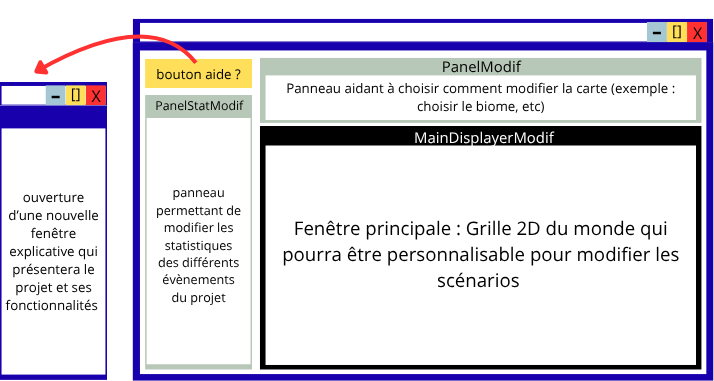
\includegraphics[width=0.9\textwidth]{images/mode_edition.png}
  \caption{Schéma conceptuel de l'interface de configuration initiale}
  \label{fig:schema_edition}
\end{figure}

\needspace{7\baselineskip}
\paragraph{Fenêtre de simulation.}
Lorsque l'utilisateur clique sur le bouton \textit{Lancer}, la fenêtre d'édition
se ferme et la fenêtre principale de simulation s'ouvre. Comme le montre la
figure~\ref{fig:fenetre_simulation}, elle est composée de trois zones
fonctionnelles.

Les trois zones visibles dans la figure~\ref{fig:fenetre_simulation} sont les
suivantes~:

\begin{itemize}
  \item la zone centrale (\texttt{MainDisplayer}) affiche la grille de simulation
    avec les biomes et les événements superposés~;
  \item le panneau latéral droit (\texttt{PanelStatistique}) présente les
    statistiques en temps réel (décompte de chaque type de biome) et les graphiques
    JFreeChart d'évolution des propriétés~;
  \item le panneau inférieur (\texttt{PanelTemps}) regroupe les contrôles de
    simulation (Play, Pause, Vitesse~$\times 2$, Bilan de fin).
\end{itemize}

La structure logique de ces contrôles de pilotage est illustrée dans la
figure~\ref{fig:schema_simulation}.

\begin{figure}[htbp]
  \centering
  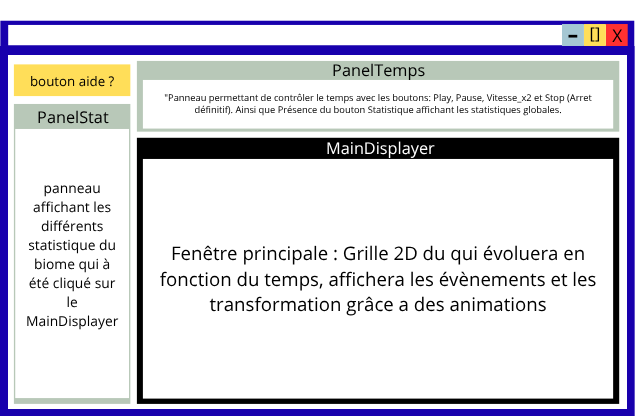
\includegraphics[width=0.85\textwidth]{images/mode_simulation.png}
  \caption{Schéma conceptuel de l'interface de pilotage dynamique}
  \label{fig:schema_simulation}
\end{figure}

\begin{figure}[htbp]
  \centering
  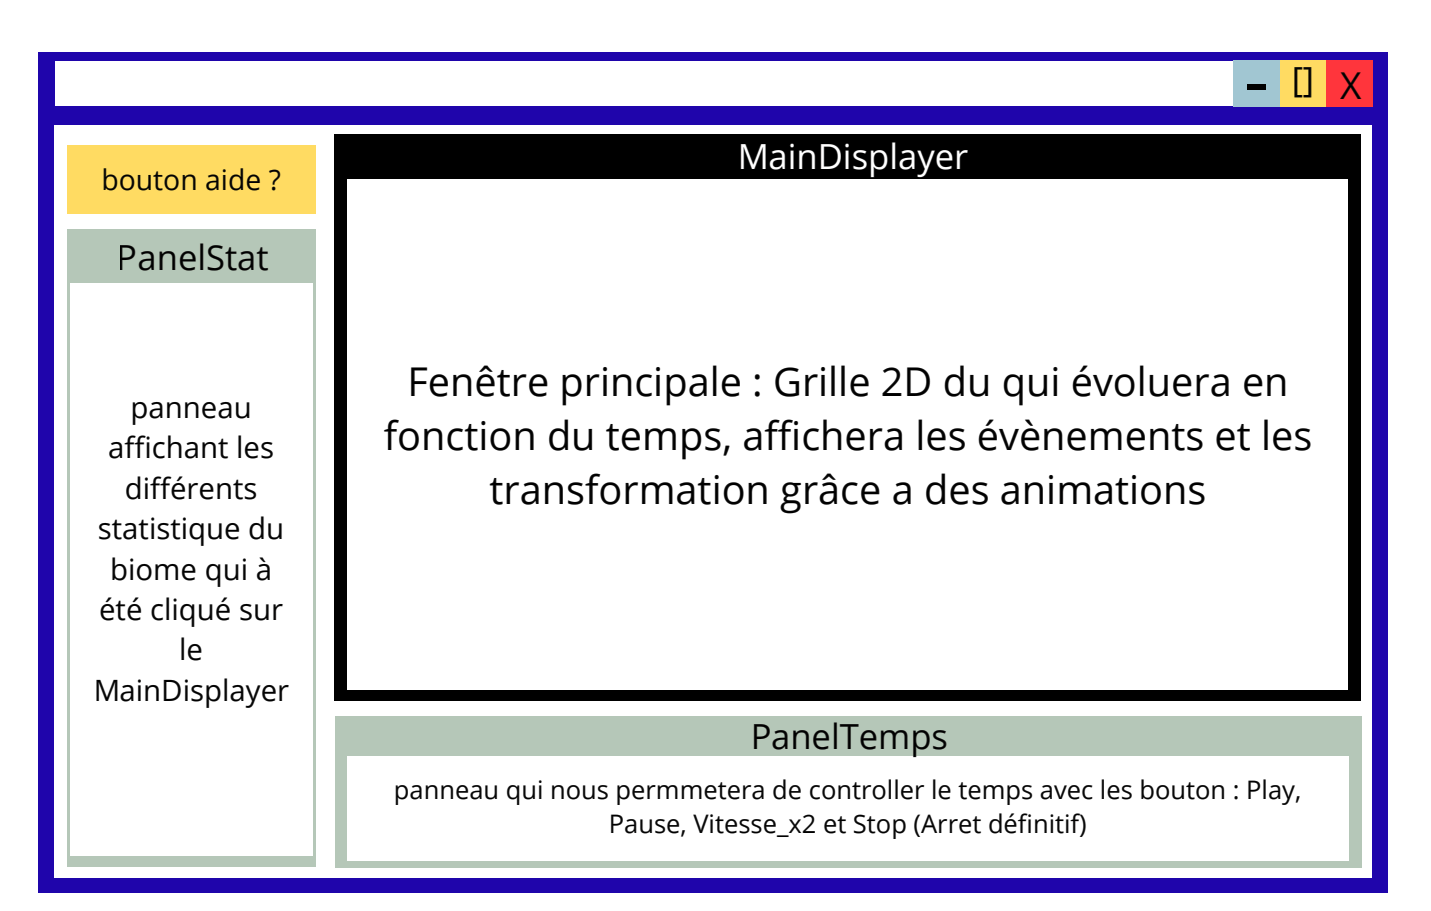
\includegraphics[width=0.9\textwidth]{images/fenetre_simulation.png}
  \caption{Fenêtre principale de simulation avec ses trois zones fonctionnelles}
  \label{fig:fenetre_simulation}
\end{figure}

\needspace{10\baselineskip}
\paragraph{Fenêtre de tutoriel.}
Afin d'améliorer l'accessibilité de l'application, une fenêtre de tutoriel a été
intégrée. Accessible depuis la fenêtre principale via un bouton dédié, elle est
implémentée par la classe \texttt{TutorielPanel} et s'affiche dans une
\texttt{JDialog} modale. Cette fenêtre présente les règles fondamentales de la
simulation~: le rôle de chaque type de biome, le comportement des événements et
la logique des transformations écologiques. L'affichage modal garantit que
l'utilisateur peut consulter ces informations contextuelles sans que la simulation
en cours ne soit interrompue ni fermée.

\begin{figure}[htbp]
  \centering
  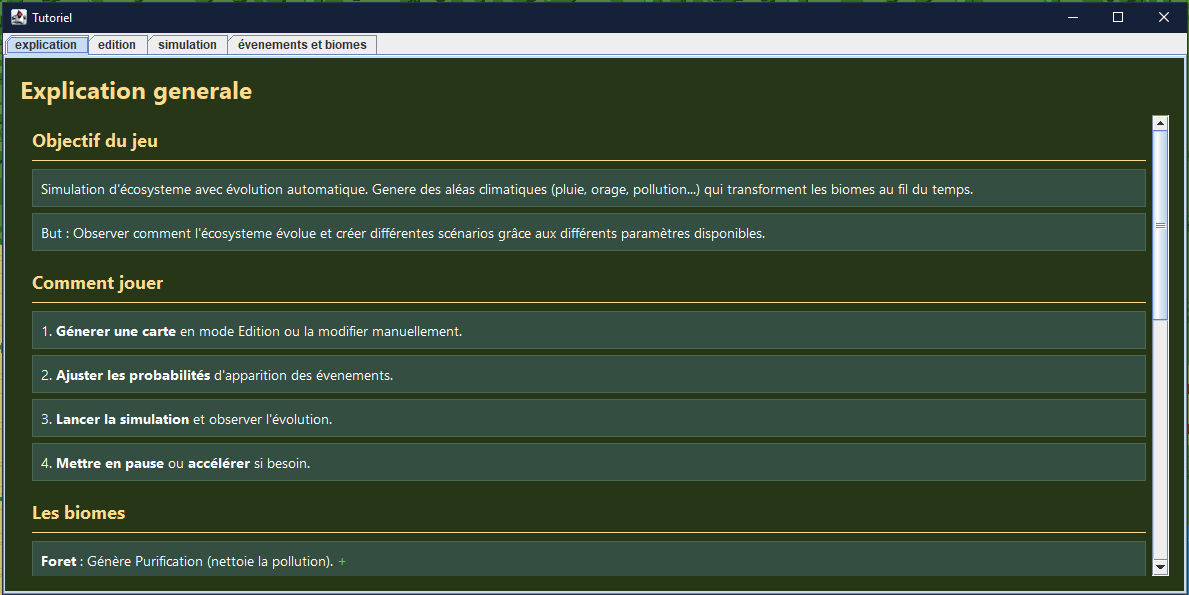
\includegraphics[width=0.9\textwidth]{images/fenetre_aide.png}
  \caption{Fenêtre de tutoriel}
  \label{fig:fenetre_aide}
\end{figure}

\paragraph{Strategy de rendu.}
La classe \texttt{StrategiePeinture} centralise le rendu graphique de l'ensemble
des éléments de la simulation. Chaque méthode \texttt{paintComponent} est
spécialisée pour dessiner un type précis de biome ou d'événement, ce qui permet
d'adapter l'apparence visuelle de chaque élément indépendamment du reste du code
d'affichage. Cette spécialisation facilite l'ajout d'un nouveau rendu graphique
sans modifier les classes de données ni le moteur de simulation.

% ------------------------------------------------------------
\needspace{8\baselineskip}
\subsection{Conception des traitements algorithmiques}
\label{subsec:traitements}

Cette sous-section détaille la logique algorithmique et mathématique du module
\texttt{moteur}. Les formules utilisées pour les transformations, la génération
de la carte et la boucle principale de simulation y sont explicitées.

\paragraph{Formules mathématiques.}
Trois formules régissent le comportement quantitatif de la simulation.

La première formule concerne la \textbf{probabilité de génération d'un événement}.
Pour chaque type d'événement, une probabilité est définie dans la classe
\texttt{ConfigurationCreationEvenement}. Un événement est généré à chaque round
si un nombre aléatoire tiré uniformément est inférieur à cette probabilité~:

\begin{equation}
  \label{eq:proba_generation}
  P(\text{génération}) = p_{\text{configurée}}.
\end{equation}

La formule~\ref{eq:proba_generation} permet de contrôler finement la fréquence
d'apparition de chaque type d'événement.

L'équation~\ref{eq:impact} décrit le \textbf{calcul des impacts sur les propriétés}.
Lorsqu'un événement affecte un biome, ses propriétés sont mises à jour par
addition~:

\begin{equation}
  \label{eq:impact}
  p_{\text{nouvelle}} = p_{\text{actuelle}} + \Delta p_{\text{événement}}.
\end{equation}

L'équation~\ref{eq:bornage} assure le \textbf{bornage des valeurs}. Toutes les propriétés
sont contraintes dans l'intervalle $[0, 100]$ pour garantir la cohérence des
données~:

\begin{equation}
  \label{eq:bornage}
  p_{\text{bornée}} = \max\!\left(0,\; \min\!\left(100,\; p\right)\right).
\end{equation}

En Java, la formule~\ref{eq:bornage} est implémentée via les méthodes
\texttt{Math.max} et \texttt{Math.min}, appliquées systématiquement après chaque
mise à jour de propriété.

\needspace{7\baselineskip}
\paragraph{Algorithme de la boucle de simulation.}
L'algorithme principal est implémenté dans la méthode
\texttt{ManageurBasique.nextRound()}. Il exécute un cycle complet à chaque round
selon la séquence décrite dans le listing~\ref{lst:nextrond}.

\begin{lstlisting}[style=algo, label=lst:nextrond,
    caption={Pseudo-code de la méthode nextRound()}]
ALGORITHME nextRound()
  GENERER nouveaux evenements aleatoires
  POUR CHAQUE evenement mobile FAIRE
    CHOISIR direction aleatoire
    DEPLACER evenement d'une case
    SI deplacement bloque (Montagne) ALORS
      CHOISIR nouvelle direction aleatoire
    FIN SI
    APPLIQUER impacts sur le biome cible
  FIN POUR CHAQUE
  POUR CHAQUE biome de la carte FAIRE
    EVALUER toutes les regles de transformation
    SI conditions d'une regle remplies ALORS
      TRANSFORMER biome selon la regle
    FIN SI
  FIN POUR CHAQUE
FIN ALGORITHME
\end{lstlisting}

L'algorithme présenté dans le listing~\ref{lst:nextrond} garantit que les quatre
étapes de la simulation sont exécutées dans un ordre déterministe à chaque round.

\needspace{20\baselineskip}
\paragraph{Algorithme de génération de la carte.}
La génération cohérente des biomes est implémentée dans
\texttt{BiomeFactory.creerBiomesCoherents()}. Cet algorithme crée une distribution
géographiquement plausible, avec des masses d'eau, des zones désertiques et des
zones urbaines, comme le présente le listing~\ref{lst:gencarte}.

\begin{lstlisting}[style=algo, label=lst:gencarte,
    caption={Pseudo-code de la génération cohérente de la carte}]
ALGORITHME creerBiomesCoherents()
  GENERER masse d'eau (forme aleatoire : coin, haut ou milieu)
  POUR CHAQUE case de la grille FAIRE
    CALCULER distance a la masse d'eau par BFS
  FIN POUR
  POUR CHAQUE case proche de l'eau ET loin d'une zone desertique FAIRE
    AFFECTER biome Village
  FIN POUR
  POUR CHAQUE case loin de l'eau ET en zone desertique FAIRE
    AFFECTER biome Desert
  FIN POUR
  POUR CHAQUE case en zone urbaine FAIRE
    AFFECTER biome Ville
  FIN POUR
  RETOURNER carte avec biomes coherents
FIN ALGORITHME
\end{lstlisting}

Les distances à la masse d'eau utilisées dans le listing~\ref{lst:gencarte} sont
calculées par propagation BFS (\textit{Breadth-First Search}), algorithme de
parcours en largeur~\cite{cormen2009intro}, pour déterminer les zones propices à
chaque type de biome.

\paragraph{Règles de transformation écologique.}
Six règles implémentent l'interface \texttt{RegleTransformation}. Chaque règle
évalue les propriétés d'un biome (température, humidité, pollution, purification)
et retourne un nouveau biome si les conditions définies dans le
tableau~\ref{tab:transformations} sont satisfaites. Les règles implémentées
sont~: Inondation, Glaciation, Désertification, Forestation, Civilisation et
Densification. Chaque règle encapsule ses conditions dans une méthode
\texttt{appliquer(Biome b)} qui retourne le biome cible ou \texttt{null} si les
conditions ne sont pas réunies~; le moteur applique simplement le premier résultat
non nul.

\needspace{7\baselineskip}
\paragraph{Génération d'événements depuis les biomes.}
La classe \texttt{EvenementFactory} crée des événements selon des probabilités
configurées dans \texttt{ConfigurationCreationEvenement}. Le patron Visiteur est
incarné par la classe \texttt{GenerateurEvenementVisitor}, qui parcourt la carte et
génère des événements supplémentaires depuis certains biomes (par exemple, un biome
Mer génère périodiquement un événement Pluie selon son identité propre). Les
probabilités de génération et les formations spatiales des événements sont
entièrement définies dans le module \texttt{config}, ce qui permet de les modifier
sans recompiler la logique métier.

\paragraph{Système de journalisation.}
Le système repose sur la bibliothèque Log4j~\cite{apache_log4j}. La classe
utilitaire \texttt{LoggerUtility} fournit un accès centralisé au logger de
l'application~; elle est conçue pour être utilisée statiquement depuis n'importe
quel module. Les journaux sont émis aux niveaux \texttt{DEBUG} et \texttt{INFO},
et écrits simultanément vers la console et vers le fichier
\texttt{src/logs/simulation.log}. Les actions journalisées incluent notamment le
démarrage et la fin de chaque round, les déplacements d'événements, les
transformations de biomes et les anomalies détectées lors de l'exécution.

\paragraph{Gestion des statistiques.}
L'affichage des statistiques en temps réel repose sur la bibliothèque
JFreeChart~\cite{jfreechart}. Les données collectées à chaque round (répartition
des biomes, évolution des propriétés moyennes) sont injectées dans des
\texttt{XYSeriesCollection} qui alimentent les graphiques du
\texttt{PanelStatistique}. Ce mécanisme permet de visualiser l'évolution temporelle
de l'écosystème avec une précision et une lisibilité supérieures aux représentations
visuelles purement symboliques.
